%!TEX root = ../paper.tex
We compare the performance of the shape-adaptive method with that of the Modified Breiman Estimator, on simulated datasets with known density fields. This allows us to test how well the proposed method can recover simple density distributions. We distinguish two types of datasets: datasets consisting of a single Gaussian distribution and noise, discussed in \cref{s:experiment:singlesphere} and datasets containing multiple Gaussian distributions next to noise, these are presented in \cref{s:experiment:multisphere}.

To quantify the performance of the estimators we use the \mse (\MSE):
\begin{equation*}
	\varMSE{\varEstimatedDensityFunction{\bullet}} = \frac{1}{\varNumPatterns} \sum_{\itXs = 1}^{\varNumPatterns} {\left(\varEstimatedDensityFunction{\varPattern[\itXs]} - \varDensityFunction{\varPattern[\itXs]} \right)}^2.
\end{equation*}

\subsection{Datasets with a Single Gaussian}
\label{s:experiment:singlesphere}
%!TEX root = ../paper.tex

\begin{figure}
	\centering
	\begin{subfigure}{0.23\textwidth}
		\centering
		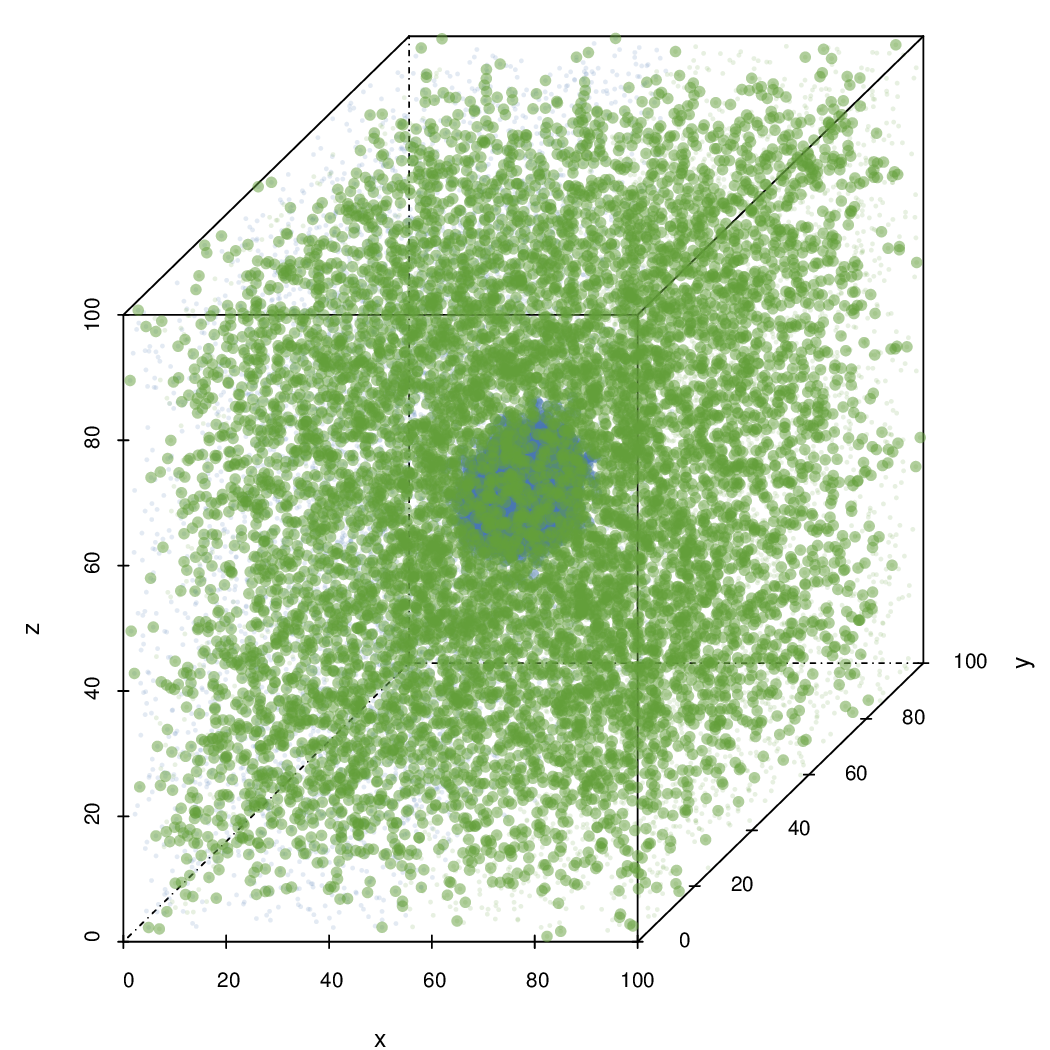
\includegraphics[keepaspectratio=true, width=\textwidth, height=0.23\textheight]{discussion/img/ferdosi_1_abs_error_mbeSmallerThansambe}
		\caption{Dataset \ferdosiOne}
		\label{fig:discussion:singleSphere:mbeLowerError:ferdosi1}
	\end{subfigure}
	\begin{subfigure}{0.23\textwidth}
		\centering
		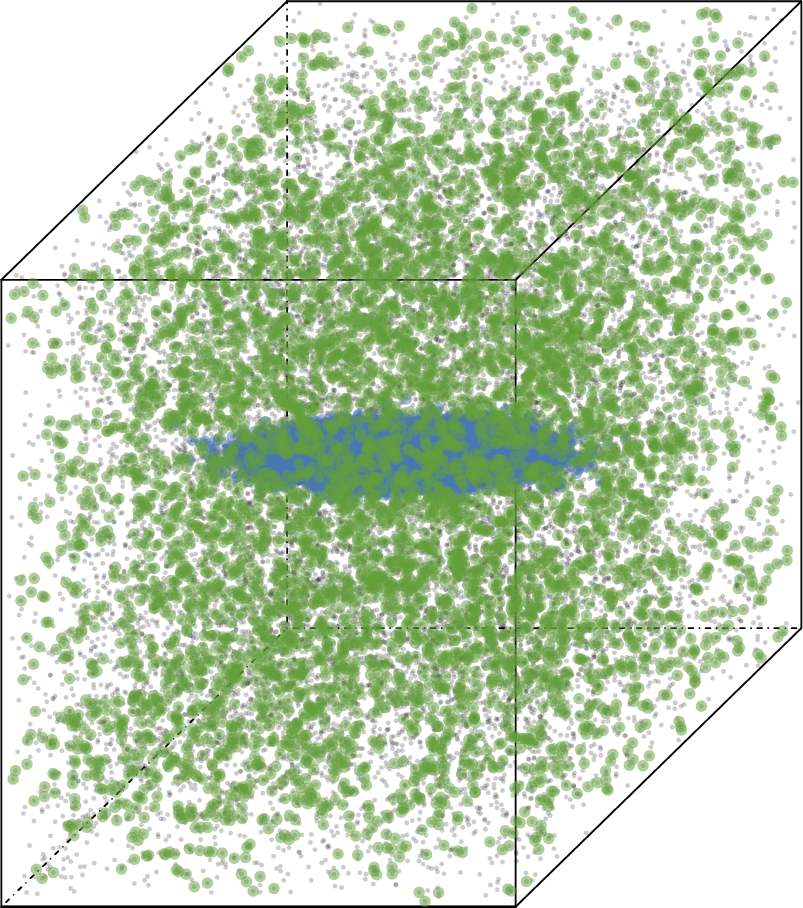
\includegraphics[keepaspectratio=true, width=\textwidth, height=0.23\textheight]{discussion/img/baakman_1_abs_error_mbeSmallerThansambe}
		\caption{Dataset \baakmanOne}
		\label{fig:discussion:singleSphere:mbeLowerError:baakman1}
	\end{subfigure}	
	\begin{subfigure}{0.23\textwidth}
		\centering
		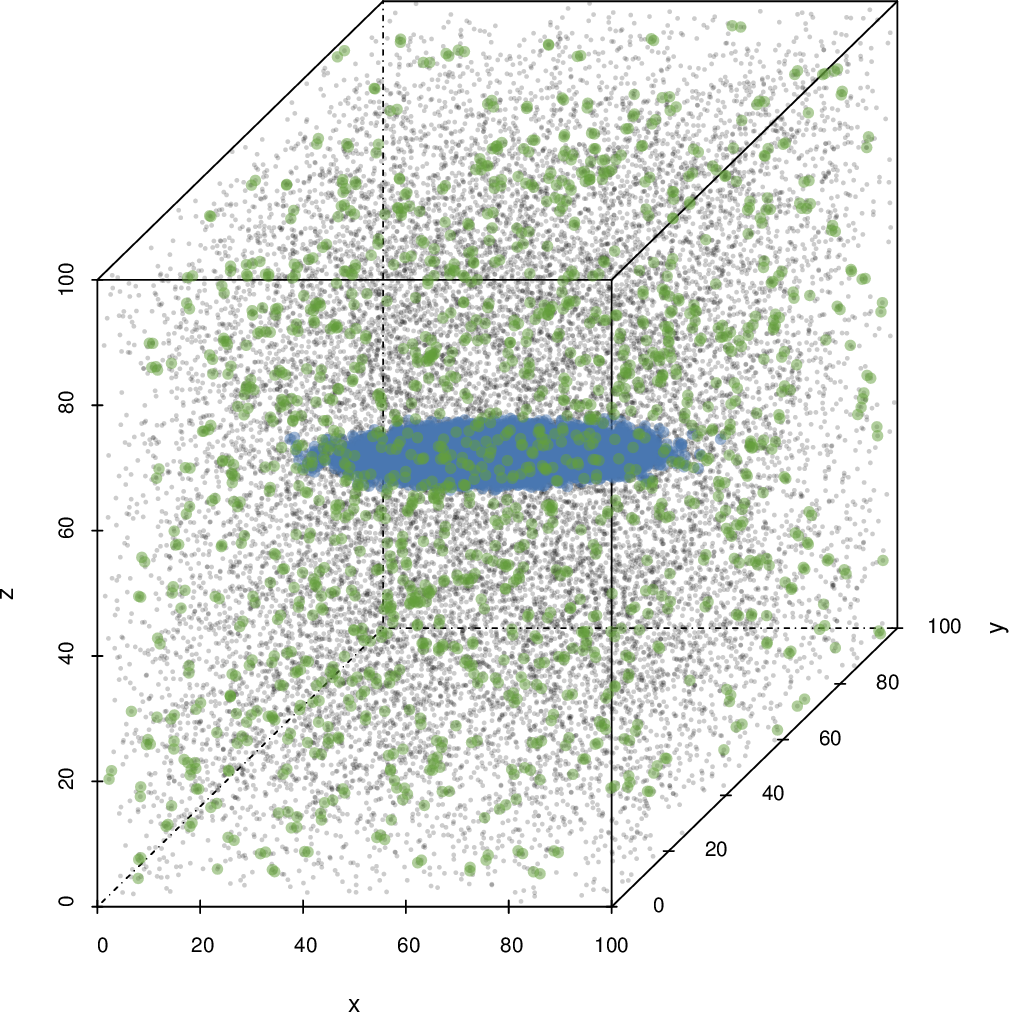
\includegraphics[keepaspectratio=true, width=\textwidth, height=0.23\textheight]{discussion/img/baakman_4_abs_error_mbeSmallerThansambe}
		\caption{Dataset \baakmanFour}
		\label{fig:discussion:singleSphere:mbeLowerError:baakman4}
	\end{subfigure}		
	\begin{subfigure}{0.23\textwidth}
		\centering
		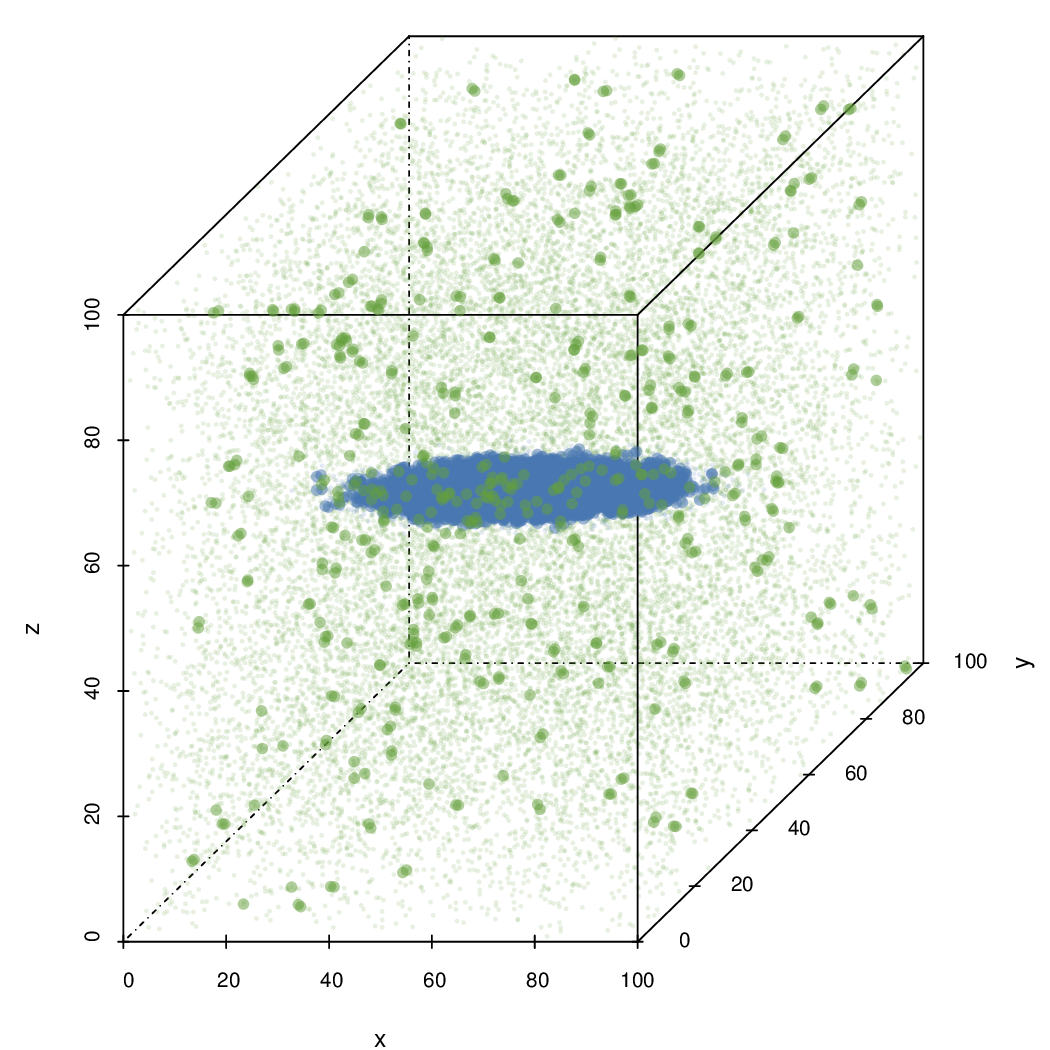
\includegraphics[keepaspectratio=true, width=\textwidth, height=0.23\textheight]{discussion/img/baakman_5_abs_error_mbeSmallerThansambe}
		\caption{Dataset \baakmanFive}
		\label{fig:discussion:singleSphere:mbeLowerError:baakman5}
	\end{subfigure}			
	\caption{Low opacity scatter plot of dataset %
		\subref{fig:discussion:singleSphere:mbeLowerError:ferdosi1} \ferdosiOne, %
		\subref{fig:discussion:singleSphere:mbeLowerError:baakman1} \baakmanOne, %
		\subref{fig:discussion:singleSphere:mbeLowerError:baakman4} \baakmanFour, and%
		\subref{fig:discussion:singleSphere:mbeLowerError:baakman5} \baakmanFive, %
		with an overlay of larger points with a higher opacity where the absolute error of \sambe is larger than or equal to the absolute error of \mbe.}
	\label{fig:discussion:singleSphere:mbeLowerError}
\end{figure}

% Introduction
The scatter plots of the datasets with a single Gaussian in \cref{fig:discussion:singleSphere:mbeLowerError} emphasize the points where the absolute error of the symmetric estimator is smaller than that of the shape-adaptive estimator. 

	% Ferdosi 1
		% ALl POINTS
		% SAMBE better than MBE: 2.828800000000000e+04 (4.727588742563005e+01 percent)
		% MBE better than SAMBE: 3.154800000000000e+04 (5.272411257436994e+01 percent)
		% MBE equal to SAMBE: 0.000000000000000e+00 (0.000000000000000e+00 percent)
		
		% Component 0
		% MSE(MBE, SAMBE):
		%  1.245351981191544e-08	& 1.335673957702697e-08

		% SAMBE better than MBE: 1.773700000000000e+04 (4.434250000000000e+01 percent)
		% MBE better than SAMBE: 2.226300000000000e+04 (5.565750000000001e+01 percent)
		% MBE equal to SAMBE: 0.000000000000000e+00 (0.000000000000000e+00 percent)

		% Component 1
		% MSE(MBE, SAMBE):
		%  1.046361645486837e-11	& 1.282383835662826e-11

		% SAMBE better than MBE: 1.055100000000000e+04 (5.319116757410768e+01 percent)
		% MBE better than SAMBE: 9.285000000000000e+03 (4.680883242589232e+01 percent)
		% MBE equal to SAMBE: 0.000000000000000e+00 (0.000000000000000e+00 percent)	


		% The overlay plot
		\Cref{fig:discussion:singleSphere:mbeLowerError:ferdosi1} shows that the shape-adaptive estimator results outperforms the symmetric estimators on most points near the boundary of the dataset. It also seems to illustrate that that \mbe results in a lower error than \sambe on the other points, however the raw data shows that on \SI{5.272411257436994e+01}{\percent} of the full dataset, and on \SI{5.565750000000001e+01}{\percent} of the Gaussian component the symmetric estimator results in a lower absolute error.
		% The shape of the kernels
		Reviewing the shape of the kernels used for the points in dataset \ferdosiOne we find that the used kernels are all near spherical. The kernels with the largest differences between their eigenvalues are associated with points near the boundary of the dataset. 
		% Largest differnces in estimated values between kernels. 
		The largest differences in error between the two estimators can be found near the mean of the Gaussian component, where the shape-adaptive kernels are relatively spherical. We think it likely that the difference between the two estimators at these points is caused by the difference in physical density at that location in the dataset, which ensures that a kernel that is slightly elliptical has a result that differs strongly from that of a spherical kernel. This is confirmed by the large differences in the number of patterns that are used in the density estimate of the points near the mean of the Gaussian component between the two estimators. 

	% Baakman 1
		% Component -1
		% MSE(MBE, SAMBE):
		%  1.494313211797496e-08	& 1.544094229246398e-08
		% SAMBE better than MBE: 2.509400000000000e+04 (4.193796376763152e+01 percent)
		% MBE better than SAMBE: 2.680000000000000e+04 (4.478909017982485e+01 percent)
		% MBE equal to SAMBE: 7.942000000000000e+03 (1.327294605254362e+01 percent)

		% Component 0
		% MSE(MBE, SAMBE):
		%  2.231981590358483e-08	& 2.306388047782812e-08
		% SAMBE better than MBE: 1.924800000000000e+04 (4.812000000000000e+01 percent)
		% MBE better than SAMBE: 2.061300000000000e+04 (5.153250000000001e+01 percent)
		% MBE equal to SAMBE: 1.390000000000000e+02 (3.475000000000000e-01 percent)

		% Component 1
		% MSE(MBE, SAMBE):
		%  6.778671444628963e-11	& 6.901612718035766e-11
		% SAMBE better than MBE: 5.846000000000000e+03 (2.947166767493447e+01 percent)
		% MBE better than SAMBE: 6.187000000000000e+03 (3.119076426698931e+01 percent)
		% MBE equal to SAMBE: 7.803000000000000e+03 (3.933756805807623e+01 percent)

		% Overlay plot
		The results in \cref{fig:discussion:singleSphere:mbeLowerError:baakman1} are comparable to those in \cref{fig:experiment:singlesphere:ferdosi1}, however fewer points of the noise component seem to emphasized in the former. This would mean that the absolute error for most points of the noise component is lower when using symmetric kernels instead of shape-adaptive kernels. Reviewing the raw data shows that this difference is primarily caused by the \num{7.803000000000000e+03} points for which both estimators estimate the same density. We expect that this is due to the elongated shape of the distribution, as its shape influences the kernel of fewer points of the noise component, resulting in more spherical kernels, which causes the estimators to give the same estimate.
		% The shape of the kernels
		As in dataset \ferdosiOne the points with the most ellipsoidal kernels are positioned near the boundaries of the dataset, where \sambe outperforms \mbe. 
		% Largest differences in estiamted values between estimators
		The points whose differences in estimated densities are largest are, as in dataset \ferdosiOne, found near the mean of the Gaussian distribution. We hypothesize that this is occurs in this dataset for the same reason as it occurs in dataset \ferdosiOne.

	%Baakman 4
		% Component -1
		% MSE(MBE, SAMBE):
		%  2.945143538188240e-08	& 2.971553835946330e-08

		% SAMBE better than MBE: 2.061700000000000e+04 (3.445584597900929e+01 percent)
		% MBE better than SAMBE: 2.132900000000000e+04 (3.564576509124942e+01 percent)
		% MBE equal to SAMBE: 1.789000000000000e+04 (2.989838892974129e+01 percent)	
		% Component 0
		% MSE(MBE, SAMBE):
		%  4.404296246131644e-08	& 4.443607459199309e-08

		% SAMBE better than MBE: 1.926500000000000e+04 (4.816250000000000e+01 percent)
		% MBE better than SAMBE: 1.988200000000000e+04 (4.970500000000000e+01 percent)
		% MBE equal to SAMBE: 8.530000000000000e+02 (2.132500000000000e+00 percent)


		% Component 1
		% MSE(MBE, SAMBE):
		%  2.710168671393879e-11	& 3.105311540244085e-11

		% SAMBE better than MBE: 1.352000000000000e+03 (6.815890300463804e+00 percent)
		% MBE better than SAMBE: 1.447000000000000e+03 (7.294817503528937e+00 percent)
		% MBE equal to SAMBE: 1.703700000000000e+04 (8.588929219600726e+01 percent)	
	
		% Overlay Plot
		In \cref{fig:discussion:singleSphere:mbeLowerError:baakman4} we observe that the \mbe outperforms \sambe on very few points in dataset \baakmanFour, to be exact on \num{92.7051824965} percent of the points the absolute error of the shape-adaptive estimator was at least as low as that of the symmetric estimator. We expect that the effect of the Gaussian component is stronger than in dataset \baakmanOne since it is more elongated.
		% Shape of the kernels
		Reviewing the shape of the kernels we find kernels with large differences between their eigenvalues both near the boundary of the dataset, where \sambe outperforms \mbe, and near the Gaussian component. We expect that the last occurs in this dataset and not in set \baakmanOne due to how much more elongated the Gaussian component is. 
		% Largest differences in estimated values between estimators
		Near the mean of this component we also find the biggest differences in estimated densities between the two estimators.

	%Baakman 5
		% Component -1
		% MSE(MBE, SAMBE):
		%  5.587052323057813e-08	& 5.600040277292591e-08

		% SAMBE better than MBE: 1.935100000000000e+04 (3.234006283842503e+01 percent)
		% MBE better than SAMBE: 1.933100000000000e+04 (3.230663814426098e+01 percent)
		% MBE equal to SAMBE: 2.115400000000000e+04 (3.535329901731399e+01 percent)

		% Component 0
		% MSE(MBE, SAMBE):
		%  8.350875457323442e-08	& 8.370053660739159e-08
		% SAMBE better than MBE: 1.892300000000000e+04 (4.730750000000000e+01 percent)
		% MBE better than SAMBE: 1.884700000000000e+04 (4.711750000000000e+01 percent)
		% MBE equal to SAMBE: 2.230000000000000e+03 (5.575000000000000e+00 percent)


		% Component 1
		% MSE(MBE, SAMBE):
		%  1.370460322391959e-10	& 1.420969966289269e-10
		% SAMBE better than MBE: 4.280000000000000e+02 (2.157693083282920e+00 percent)
		% MBE better than SAMBE: 4.840000000000000e+02 (2.440008066142367e+00 percent)
		% MBE equal to SAMBE: 1.892400000000000e+04 (9.540229885057471e+01 percent)	

		% Overlay plot
		The effect of how elongated the Gaussian component is on how well the density of the noise is estimated is stronger in dataset \baakmanFive, as illustrated in \cref{fig:discussion:singleSphere:mbeLowerError:baakman5}. The density estimate of the two estimates is the same for \SI{9.540229885057471e+01}{\percent} of the points drawn from the uniform distribution, contrastingly this is only the case for \SI{5.575000000000000e+00}{\percent} of the points from the Gaussian component. 
		% Shape of the Kernels
		As in dataset \baakmanFour the shape of the kernels is most strongly influenced by the data near the boundaries of the dataset and the Gaussian component.
		% Largest differences in estimated values between estimators
		The largest differences between the results of the two estimators are, comparable to what we observed in dataset \baakmanFour, found near the mean of the Gaussian component. 

% General observations 
% Strong difference in kernel shape near the Gaussian in baakman 4 and 5
In general we have found that if the Gaussian component is strongly elongated, as in dataset \baakmanFour and \baakmanFive, the shape of the kernels near the mean of the Gaussian component is influenced, whereas the spherical and ellipsoidal Gaussian component in dataset \ferdosiOne and \baakmanOne, respectively, hardly influences the shape of the kernels of the data points near its mean. We expect that this is caused by a lower physical density of points near the means of the more spherical Gaussians. 
% Strong difference in density estimate near the mean of the Gaussian in ferdosi 1, baakman 1, baakman 4, baakman 5
In spite of this difference between the four datasets, in all datasets the difference in estimated density between the estimators is largest near the mean of the Gaussian component. We expect that this is due to the relative high density of points at this location, which causes small differences in the shapes of the kernels to have a large effect on the final density. 

\subsection{Datasets with Multiple Gaussians}
\label{s:experiment:multisphere}
%!TEX root = ../paper.tex

\begin{figure}
	\centering
	\beforeFinalVersion{Remove ticks and labels.}
	%!TEX root = ../paper.tex

% Ferdosi Set 2
\begin{subfigure}{0.23\textwidth}
	\centering
	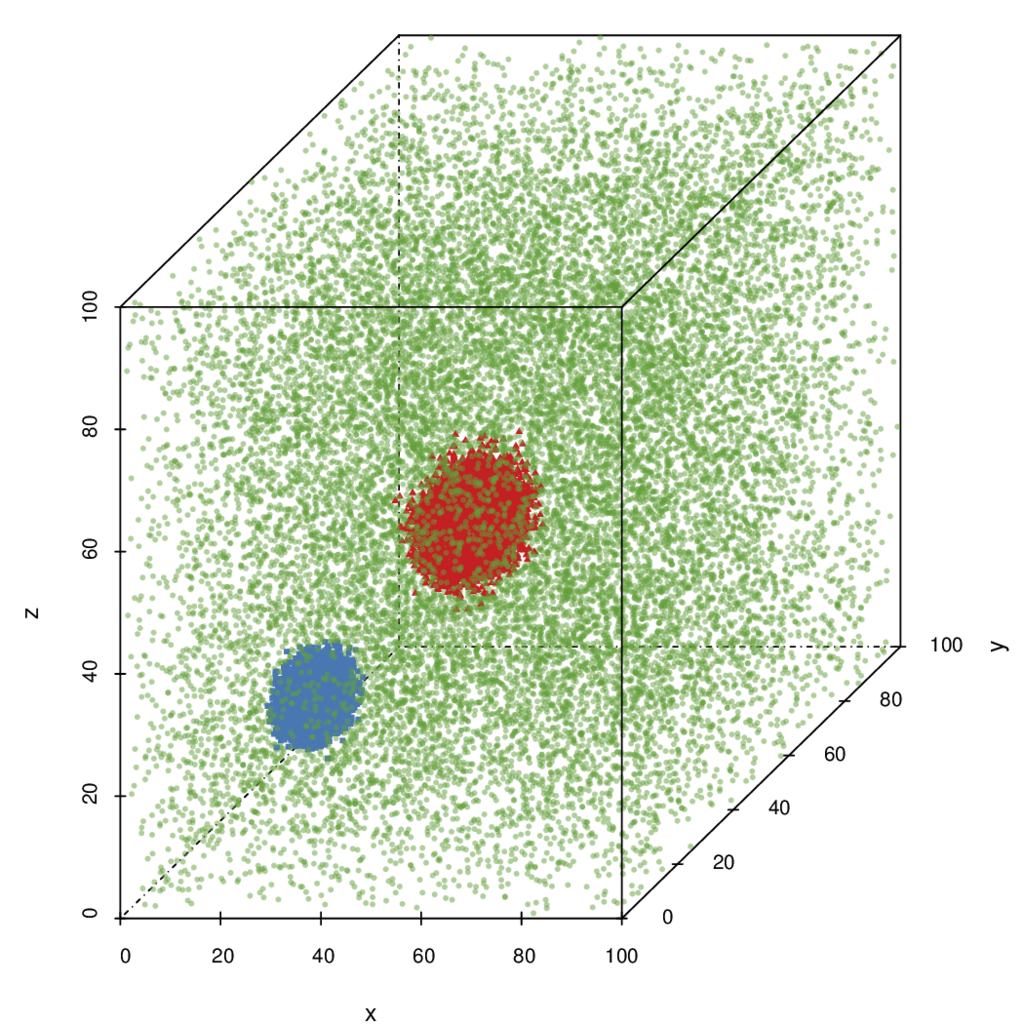
\includegraphics[width=\textwidth]{experiment/img/datasetplot_ferdosi_2_60000}
	\caption{Set \ferdosiTwo}
	\label{fig:experiment:multisphere:ferdosi2}
\end{subfigure}	
% Ferdosi Set 3
\begin{subfigure}{0.23\textwidth}
	\centering
	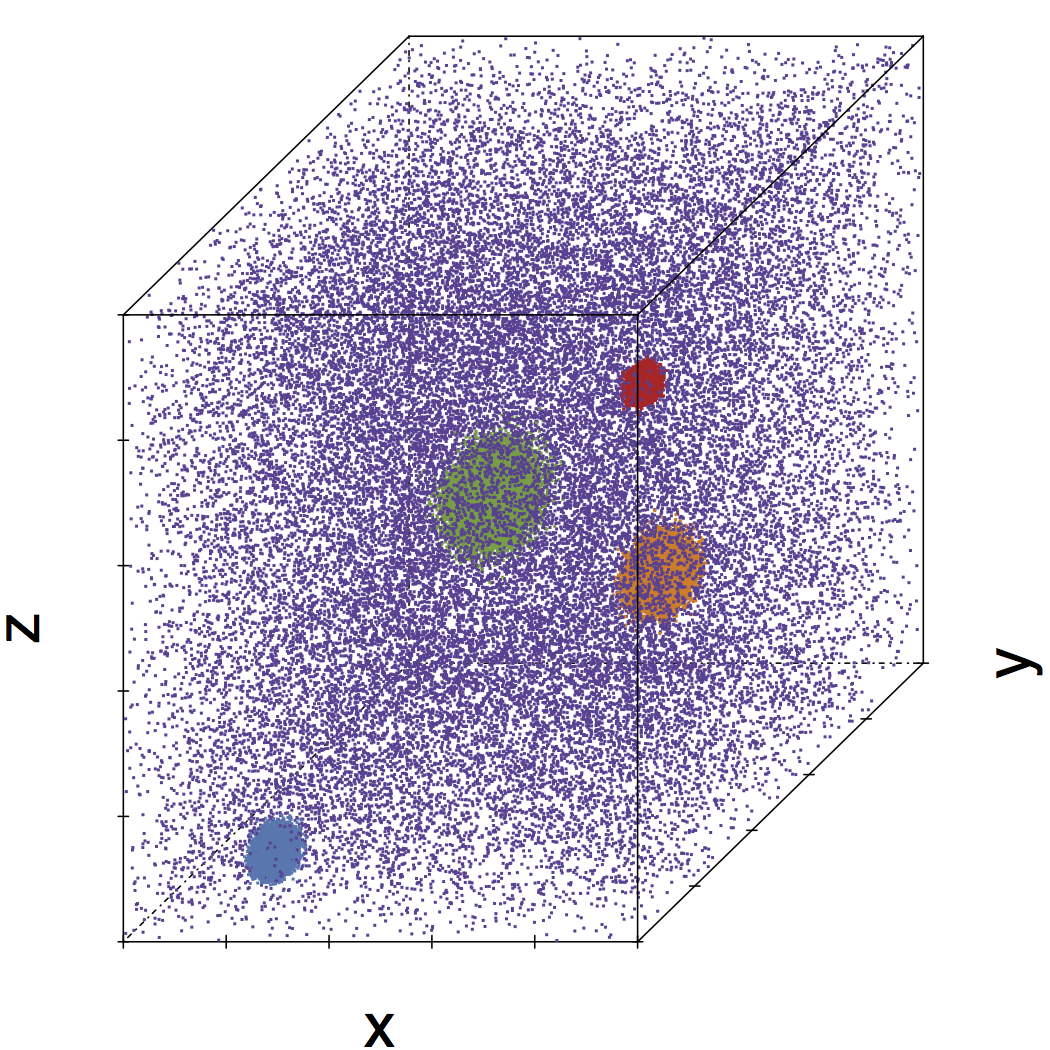
\includegraphics[width=\textwidth]{experiment/img/datasetplot_ferdosi_3_120000}
	\caption{Set \ferdosiThree}
	\label{fig:experiment:multisphere:ferdosi3}
\end{subfigure}	
% Baakman 2
\begin{subfigure}{0.23\textwidth}
	\centering
	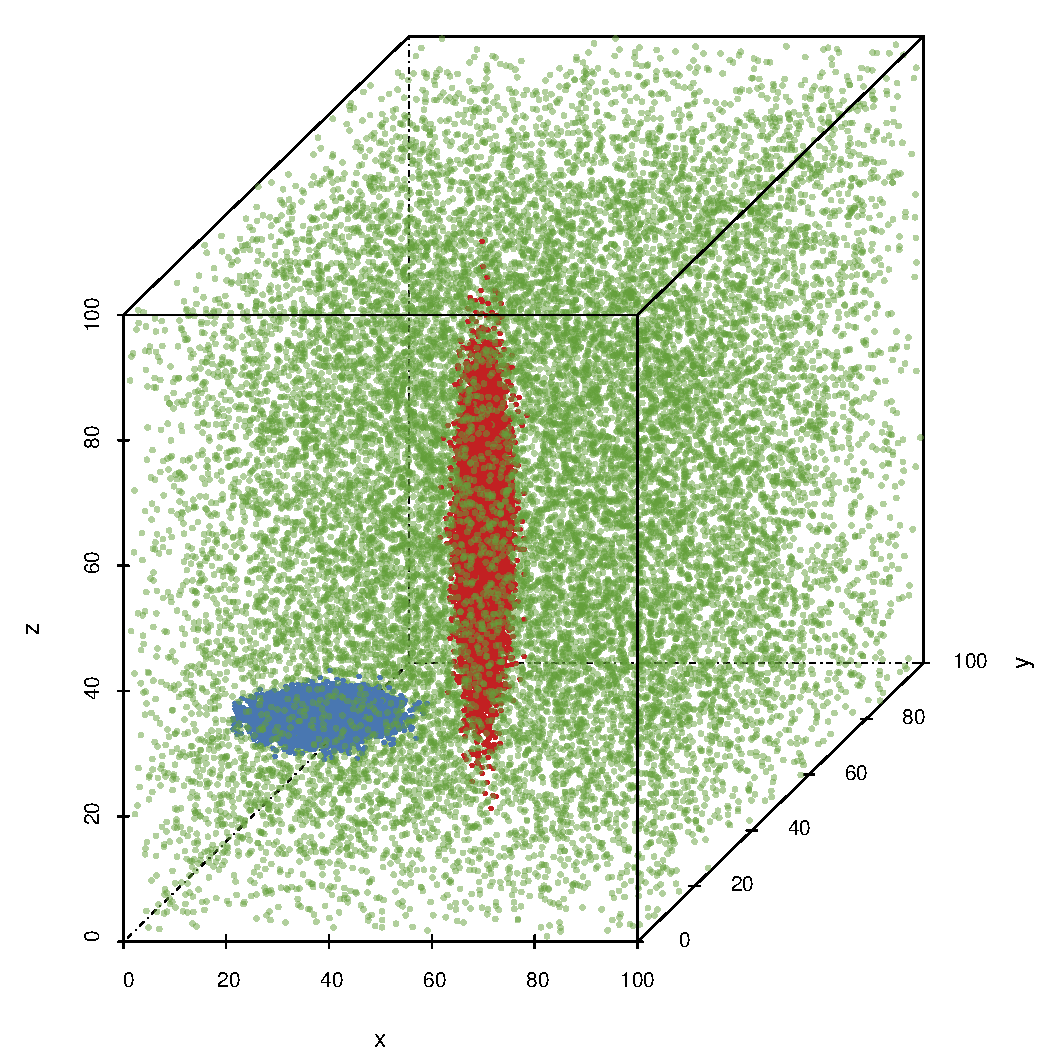
\includegraphics[width=\textwidth]{experiment/img/datasetplot_baakman_2_60000}
	\caption{Set \baakmanTwo}
	\label{fig:experiment:multisphere:baakman2}
\end{subfigure}			
% Baakman 3
\begin{subfigure}{0.23\textwidth}
	\centering
	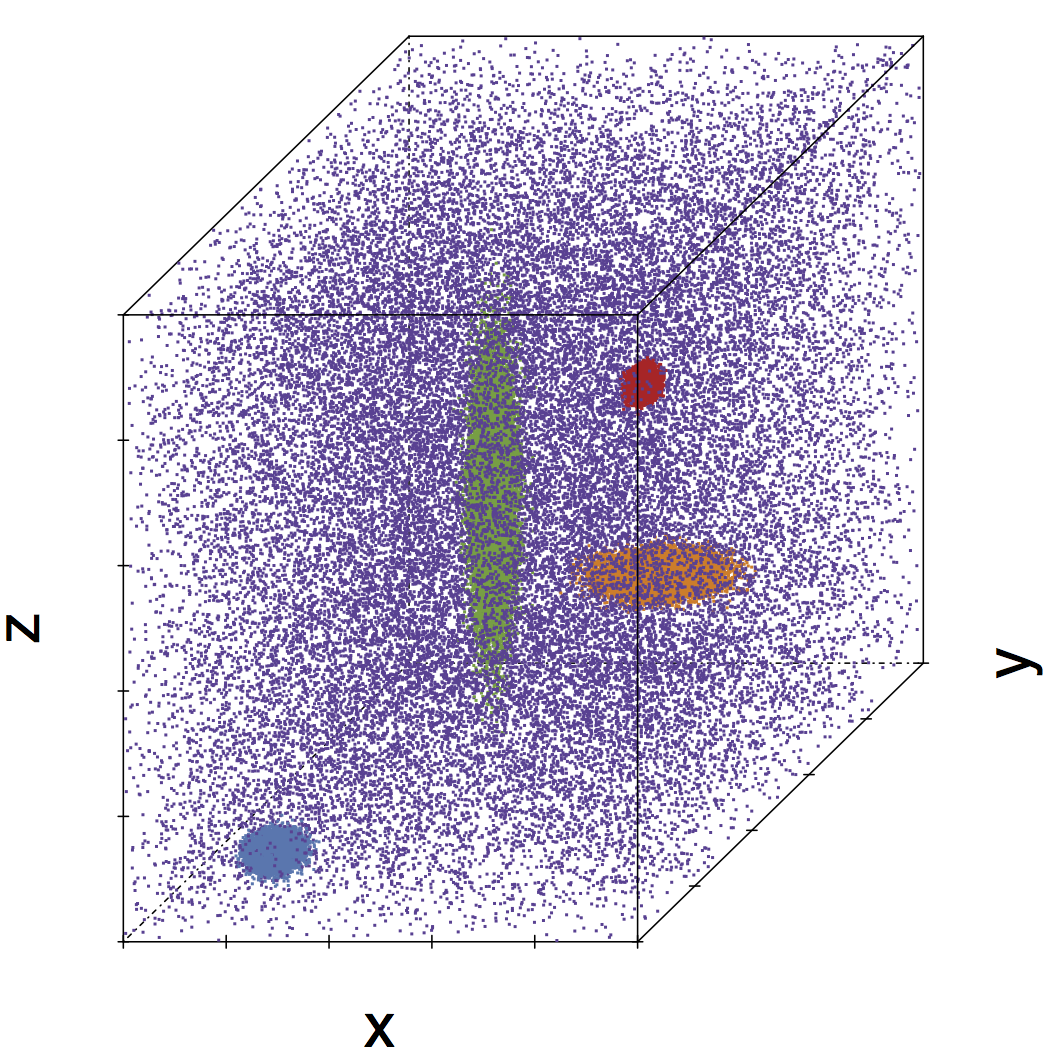
\includegraphics[width=\textwidth]{experiment/img/datasetplot_baakman_3_120000}
	\caption{Set \baakmanThree}
	\label{fig:experiment:multisphere:baakman3}
\end{subfigure}
	\caption{Scatter plot representation of the datasets defined in \cref{tab:experiment:multisphere:sets}, the colors used for the different components correspond to those in \cref{tab:experiment:multisphere:sets}.}
	\label{fig:experiment:multisphere:sets}
\end{figure}

\begin{table*}
	\centering
	%!TEX root = ../paper.tex

\begin{tabular}{@{}cclS[table-format=+1.1e+1,scientific-notation=true,round-mode=places,round-precision=1]l@{}}
\toprule
Set 			&~						& Component					& {Number} 	& Distribution\\
\midrule
% Ferdosi 2
\ferdosiTwo 	&\legendComponentOne	& Trivariate Gaussian 1		& 20000		& $\gaussDist{[25, 25, 25]}{\diag(5)}$\\
~ 				&\legendComponentTwo	& Trivariate Gaussian 2		& 20000		& $\gaussDist{[45, 45, 45]}{\diag(11)}$\\
~ 				&\legendComponentNoise	& Uniform random background	& 20000		& $\uniformDist{[0, 0, 0]}{[100, 100, 100]}$\\
% Baakman 2
\hline
\baakmanTwo		&\legendComponentOne	& Trivariate Gaussian 1		& 20000		& $\gaussDist{[25, 25, 25]}{\diag([5^2, \sqrt{5}, \sqrt{5}])}$\\
~ 				&\legendComponentTwo	& Trivariate Gaussian 2		& 20000		& $\gaussDist{[45, 45, 45]}{\diag([\sqrt{11}, \sqrt{11}, 11^2])}$\\
~ 				&\legendComponentNoise	& Uniform random background	& 20000		& $\uniformDist{[0, 0, 0]}{[100, 100, 100]}$\\
% Ferdosi 3
\hline
\ferdosiThree	&\legendComponentOne 	& Trivariate Gaussian 1 	& 20000		& $\gaussDist{[24, 10, 10]}{\diag(2)}$\\
~ 				&\legendComponentTwo	& Trivariate Gaussian 2 	& 20000		& $\gaussDist{[33, 70, 40]}{\diag(10)}$\\
~ 				&\legendComponentThree	& Trivariate Gaussian 3 	& 20000		& $\gaussDist{[90, 20, 80]}{\diag(1)}$\\
~ 				&\legendComponentFour	& Trivariate Gaussian 4 	& 20000		& $\gaussDist{[60, 80, 23]}{\diag(5)}$\\
~ 				&\legendComponentNoise	& Uniform random background	& 40000		& $\uniformDist{[0, 0, 0]}{[100, 100, 100]}$\\
% Baakman 3
\hline
\baakmanThree	&\legendComponentOne 	& Trivariate Gaussian 1 	& 20000		& $\gaussDist{[24, 10, 10]}{\diag([4, \sqrt{2}, \sqrt{2}])}$\\
~ 				&\legendComponentTwo	& Trivariate Gaussian 2 	& 20000		& $\gaussDist{[33, 70, 40]}{\diag([\sqrt{10}, \sqrt{10}, 100])}$\\
~ 				&\legendComponentThree	& Trivariate Gaussian 3 	& 20000		& $\gaussDist{[90, 20, 80]}{\diag(1)}$\\
~ 				&\legendComponentFour	& Trivariate Gaussian 4 	& 20000		& $\gaussDist{[60, 80, 23]}{\diag([25, \sqrt{5}, \sqrt{5}])}$\\
~ 				&\legendComponentNoise	& Uniform random background	& 40000		& $\uniformDist{[0, 0, 0]}{[100, 100, 100]}$\\
\bottomrule
\end{tabular}
	\caption{The datasets with multiple Gaussian distributions embedded in uniform noise. This table has the same structure and uses the same notation as \cref{tab:experiment:singlesphere:sets}.} 	
	\label{tab:experiment:multisphere:sets}
\end{table*}

%General
\Cref{tab:experiment:multisphere:sets} defines the datasets that consist of uniform random noise and multiple Gaussian distributions, a scatter plot representation of these sets is shown in \cref{fig:experiment:multisphere:sets}. 
	% Ferdosi 2
	Dataset \ferdosiTwo consists of two Gaussian distributions, that are unlikely to overlap, embedded in noise. The first Gaussian component is significantly denser than the second. 
	% Baakman 2
	The procedure outlined in \cref{s:experiment:singlesphere} for the creation of dataset \baakmanOne was used to derive dataset \baakmanTwo from \ferdosiTwo.
	% Ferdosi Three
	Dataset \ferdosiThree embeds four non-overlapping Gaussians, with eigenspheres with notably different radii, in the uniform random background. 
	%Baakman 3
	The last dataset, \baakmanThree, is a variation on \ferdosiThree, created with the method that was used for the definition of dataset \baakmanOne from \ferdosiOne. 

%Hypothesis
	Due to the spherical nature of the Gaussian components we expect hardly any difference in performance between the estimators on dataset \ferdosiTwo and \ferdosiThree. Given the shape of the Gaussian distributions embedded in dataset \baakmanTwo and \baakmanThree we hypothesize that \sambe outperforms \mbe on these sets.

\textcite{ferdosi2011comparison} found that the Modified Breiman Estimator resulted in lower Integrated Square Error if fewer Gaussian distributions were present in the datasets. Since the presented datasets are comparable to those used by \citeauthor{ferdosi2011comparison} we expect to find the same influence of the number of distributions on the error.